% Options for packages loaded elsewhere
\PassOptionsToPackage{unicode}{hyperref}
\PassOptionsToPackage{hyphens}{url}
%
\documentclass[
  ignorenonframetext,
  aspectratio=169]{beamer}
\usepackage{pgfpages}
\setbeamertemplate{caption}[numbered]
\setbeamertemplate{caption label separator}{: }
\setbeamercolor{caption name}{fg=normal text.fg}
\beamertemplatenavigationsymbolsempty
% Prevent slide breaks in the middle of a paragraph
\widowpenalties 1 10000
\raggedbottom
\setbeamertemplate{part page}{
  \centering
  \begin{beamercolorbox}[sep=16pt,center]{part title}
    \usebeamerfont{part title}\insertpart\par
  \end{beamercolorbox}
}
\setbeamertemplate{section page}{
  \centering
  \begin{beamercolorbox}[sep=12pt,center]{part title}
    \usebeamerfont{section title}\insertsection\par
  \end{beamercolorbox}
}
\setbeamertemplate{subsection page}{
  \centering
  \begin{beamercolorbox}[sep=8pt,center]{part title}
    \usebeamerfont{subsection title}\insertsubsection\par
  \end{beamercolorbox}
}
\AtBeginPart{
  \frame{\partpage}
}
\AtBeginSection{
  \ifbibliography
  \else
    \frame{\sectionpage}
  \fi
}
\AtBeginSubsection{
  \frame{\subsectionpage}
}
\usepackage{lmodern}
\usepackage{amssymb,amsmath}
\usepackage{ifxetex,ifluatex}
\ifnum 0\ifxetex 1\fi\ifluatex 1\fi=0 % if pdftex
  \usepackage[T1]{fontenc}
  \usepackage[utf8]{inputenc}
  \usepackage{textcomp} % provide euro and other symbols
\else % if luatex or xetex
  \usepackage{unicode-math}
  \defaultfontfeatures{Scale=MatchLowercase}
  \defaultfontfeatures[\rmfamily]{Ligatures=TeX,Scale=1}
\fi
\usetheme[]{Frankfurt}
\usecolortheme{beaver}
% Use upquote if available, for straight quotes in verbatim environments
\IfFileExists{upquote.sty}{\usepackage{upquote}}{}
\IfFileExists{microtype.sty}{% use microtype if available
  \usepackage[]{microtype}
  \UseMicrotypeSet[protrusion]{basicmath} % disable protrusion for tt fonts
}{}
\makeatletter
\@ifundefined{KOMAClassName}{% if non-KOMA class
  \IfFileExists{parskip.sty}{%
    \usepackage{parskip}
  }{% else
    \setlength{\parindent}{0pt}
    \setlength{\parskip}{6pt plus 2pt minus 1pt}}
}{% if KOMA class
  \KOMAoptions{parskip=half}}
\makeatother
\usepackage{xcolor}
\IfFileExists{xurl.sty}{\usepackage{xurl}}{} % add URL line breaks if available
\IfFileExists{bookmark.sty}{\usepackage{bookmark}}{\usepackage{hyperref}}
\hypersetup{
  pdftitle={Germplasm collection, conservation and utilization},
  pdfauthor={Deependra Dhakal},
  hidelinks,
  pdfcreator={LaTeX via pandoc}}
\urlstyle{same} % disable monospaced font for URLs
\newif\ifbibliography
\setlength{\emergencystretch}{3em} % prevent overfull lines
\providecommand{\tightlist}{%
  \setlength{\itemsep}{0pt}\setlength{\parskip}{0pt}}
\setcounter{secnumdepth}{-\maxdimen} % remove section numbering
\usepackage{booktabs}
\usepackage{longtable}
\usepackage{array}
\usepackage{multirow}
\usepackage{wrapfig}
\usepackage{float}
\usepackage{colortbl}
\usepackage{pdflscape}
\usepackage{tabu}
\usepackage{threeparttable}
\usepackage{threeparttablex}
\usepackage[normalem]{ulem}
\usepackage{makecell}
\usepackage{xcolor}
\usepackage{tikz} % required for image opacity change
\usepackage[absolute,overlay]{textpos} % for text formatting

% this font option is amenable for beamer
\setbeamerfont{caption}{size=\tiny}
\newlength{\cslhangindent}
\setlength{\cslhangindent}{1.5em}
\newenvironment{cslreferences}%
  {\setlength{\parindent}{0pt}%
  \everypar{\setlength{\hangindent}{\cslhangindent}}\ignorespaces}%
  {\par}

\title{Germplasm collection, conservation and utilization}
\subtitle{Conservation concept, Rate of extinction and recovery, and
National legislation on Biodiversity}
\author{Deependra Dhakal}
\date{}
\institute{Assistant Professor\\
Agriculture and Forestry University\\
\href{mailto:ddhakal.rookie@gmail.com}{\nolinkurl{ddhakal.rookie@gmail.com}}\\
\url{http://rookie.rbind.io/}}

\begin{document}
\frame{\titlepage}

\begin{frame}[allowframebreaks]
  \tableofcontents[hideallsubsections]
\end{frame}
\hypertarget{biodiversity-conservation}{%
\section{Biodiversity conservation}\label{biodiversity-conservation}}

\begin{frame}{Value of biodiversity}
\protect\hypertarget{value-of-biodiversity}{}
\footnotesize

\begin{itemize}
\tightlist
\item
  Value based on as \textbf{anthropocentric}/utilitarian approach and
  \textbf{ecocentric} approach.
\item
  Utilitarian approach assigns values for

  \begin{itemize}
  \tightlist
  \item
    aesthetics, and
  \item
    the moral responsibility of humanity to preserve natural resources
    (thus as indicator of sustainable use of resource)
  \end{itemize}
\item
  Ecocentric approach is concerned with the intrinsic value of
  biodiversity, meaning its value independent from its contribution to
  human welfare.
\item
  Direct use value as food and medicines, clothing, energy and shelter;
  items of direct use value are privately appropriable.
\item
  80\% of the people in developing countries rely on traditional
  medicine for primary health care needs.
\item
  Indirect use value: ecosystem services and templates for industrial
  products; Regulatory functions of ecosystem, nutrient recycling,
  sedimentation processes, waste treatment, water regulation etc.
\item
  Long term or option value: Value in diversity of amount of
  information, for conservation and natural evolutionary mechanism
  sustainance.
\end{itemize}
\end{frame}

\begin{frame}{What conservation entails}
\protect\hypertarget{what-conservation-entails}{}
\begin{itemize}
\tightlist
\item
  Traditional form of contribution to conservation effort due following
  peoples:

  \begin{itemize}
  \tightlist
  \item
    Geographers
  \item
    Ethnobotanists
  \item
    Plant ecologists
  \end{itemize}
\item
  Conservationists' focus has expanded from the objective of
  establishing beautiful parks and conserving select species towards a
  more holistic goal of ecosystem integrity (includes the protection of
  the existing diversity of species, natural habitats, and ecosystem
  processes).
\item
  Fundamental questions about conservation goals and strategies are:

  \begin{enumerate}
  \tightlist
  \item
    What biodiversity should be conserved; e.g., should the focus be
    particular species, ecosystems, or ecosystem services?
  \item
    Where does the targeted biodiversity occur, and where is the best
    place to protect it? and
  \item
    Given the variety of conservation tools available, which is the most
    effective method to achieve conservation objectives?
  \end{enumerate}
\end{itemize}
\end{frame}

\begin{frame}{Operational considerations}
\protect\hypertarget{operational-considerations}{}
\begin{itemize}
\tightlist
\item
  Hotspots approach to defining what should be conserved or
  coarse-filter/fine-filter approach that ensures that a given
  landscape's naturally occuring species and ecological communities are
  protected.
\item
  Identifying the appropriate conservation landscape scale (Species/taxa
  or spatial scale)
\item
  Need for multiple conservation operational tools (Governance based,
  Market based, Civil society based)
\item
  Economic evaluation and conservation trade-offs with competing
  resource demands
\item
  Use of ``easy'' tools (i.e., GIS models and remote sensing data) to
  resolve ecological features and processes and design interventions.
\end{itemize}
\end{frame}

\begin{frame}{Causes of biodiversity loss}
\protect\hypertarget{causes-of-biodiversity-loss}{}
\footnotesize

\begin{itemize}
\tightlist
\item
  It is thought that global biodiversity reached its absolute peak about
  30,000 years ago.
\item
  Antropogenic biodiversity loss is estimated at 100-1000 times higher
  than the estimated rates for natural extinction process.
\item
  Habitat loss, overexploitation, alien species introductions, building
  and mechanical constructions, and climate change have resulted in
  significant losses to biodiversity, especially over the past 50 years.
\item
  These drivers are a influential both in protected as well as open
  areas.
\item
  Within protected areas

  \begin{itemize}
  \tightlist
  \item
    range of physical (e.g., fire),
  \item
    biological (e.g., alien species),
  \item
    social (e.g., community opposition),
  \item
    political (e.g., political support),
  \item
    economic (lack of resources), and
  \item
    managerial (e.g., lack of planning) threats are faced by
    biodiversity
  \end{itemize}
\item
  Contaminiation in regenerating cross-pollinated species.
\item
  Storage conditions and handling in \emph{ex-situ}.
\item
  Restructuring or financial leanness of storage institutions.
\end{itemize}
\end{frame}

\hypertarget{risk-of-extinction}{%
\section{Risk of extinction}\label{risk-of-extinction}}

\begin{frame}{}
\protect\hypertarget{section}{}
\begin{itemize}
\tightlist
\item
  \textbf{Extinction risk}: The likelihood of extinction of a species
  with specific demographic characteristics and distribution under
  various threatening processes over time
\item
  Research has established that biodiversity is associated with
  predictable outcomes in the short term: diverse systems are less prone
  to invasion, have more stable productivity, and can be more disease
  resistant.
\item
  Diversity is associated with lower levels of contemporary extinction
  risk in birds; diverse communities provide a safe harbor for species
  that are at risk of extinction. Attributes of species (e.g., large
  body size, poor dispersal ability or small range size) can make them
  more likely to go extinct. However, it appears that the benefits
  afforded by living in a diverse community protect these
  extinction-prone species, allowing more of them to persist. (Weeks et
  al. 2022)
\end{itemize}
\end{frame}

\begin{frame}{}
\protect\hypertarget{section-1}{}
\url{https://www.un.org/sustainabledevelopment/blog/2019/05/nature-decline-unprecedented-report/}
\end{frame}

\hypertarget{methods-of-biodiversity-conservation}{%
\section{Methods of biodiversity
conservation}\label{methods-of-biodiversity-conservation}}

\begin{frame}{}
\protect\hypertarget{section-2}{}
\begin{enumerate}
\tightlist
\item
  \emph{In situ} conservation;
\item
  \emph{Ex situ} conservation;
\item
  Restoration
\end{enumerate}
\end{frame}

\begin{frame}{Gene bank}
\protect\hypertarget{gene-bank}{}
\begin{figure}
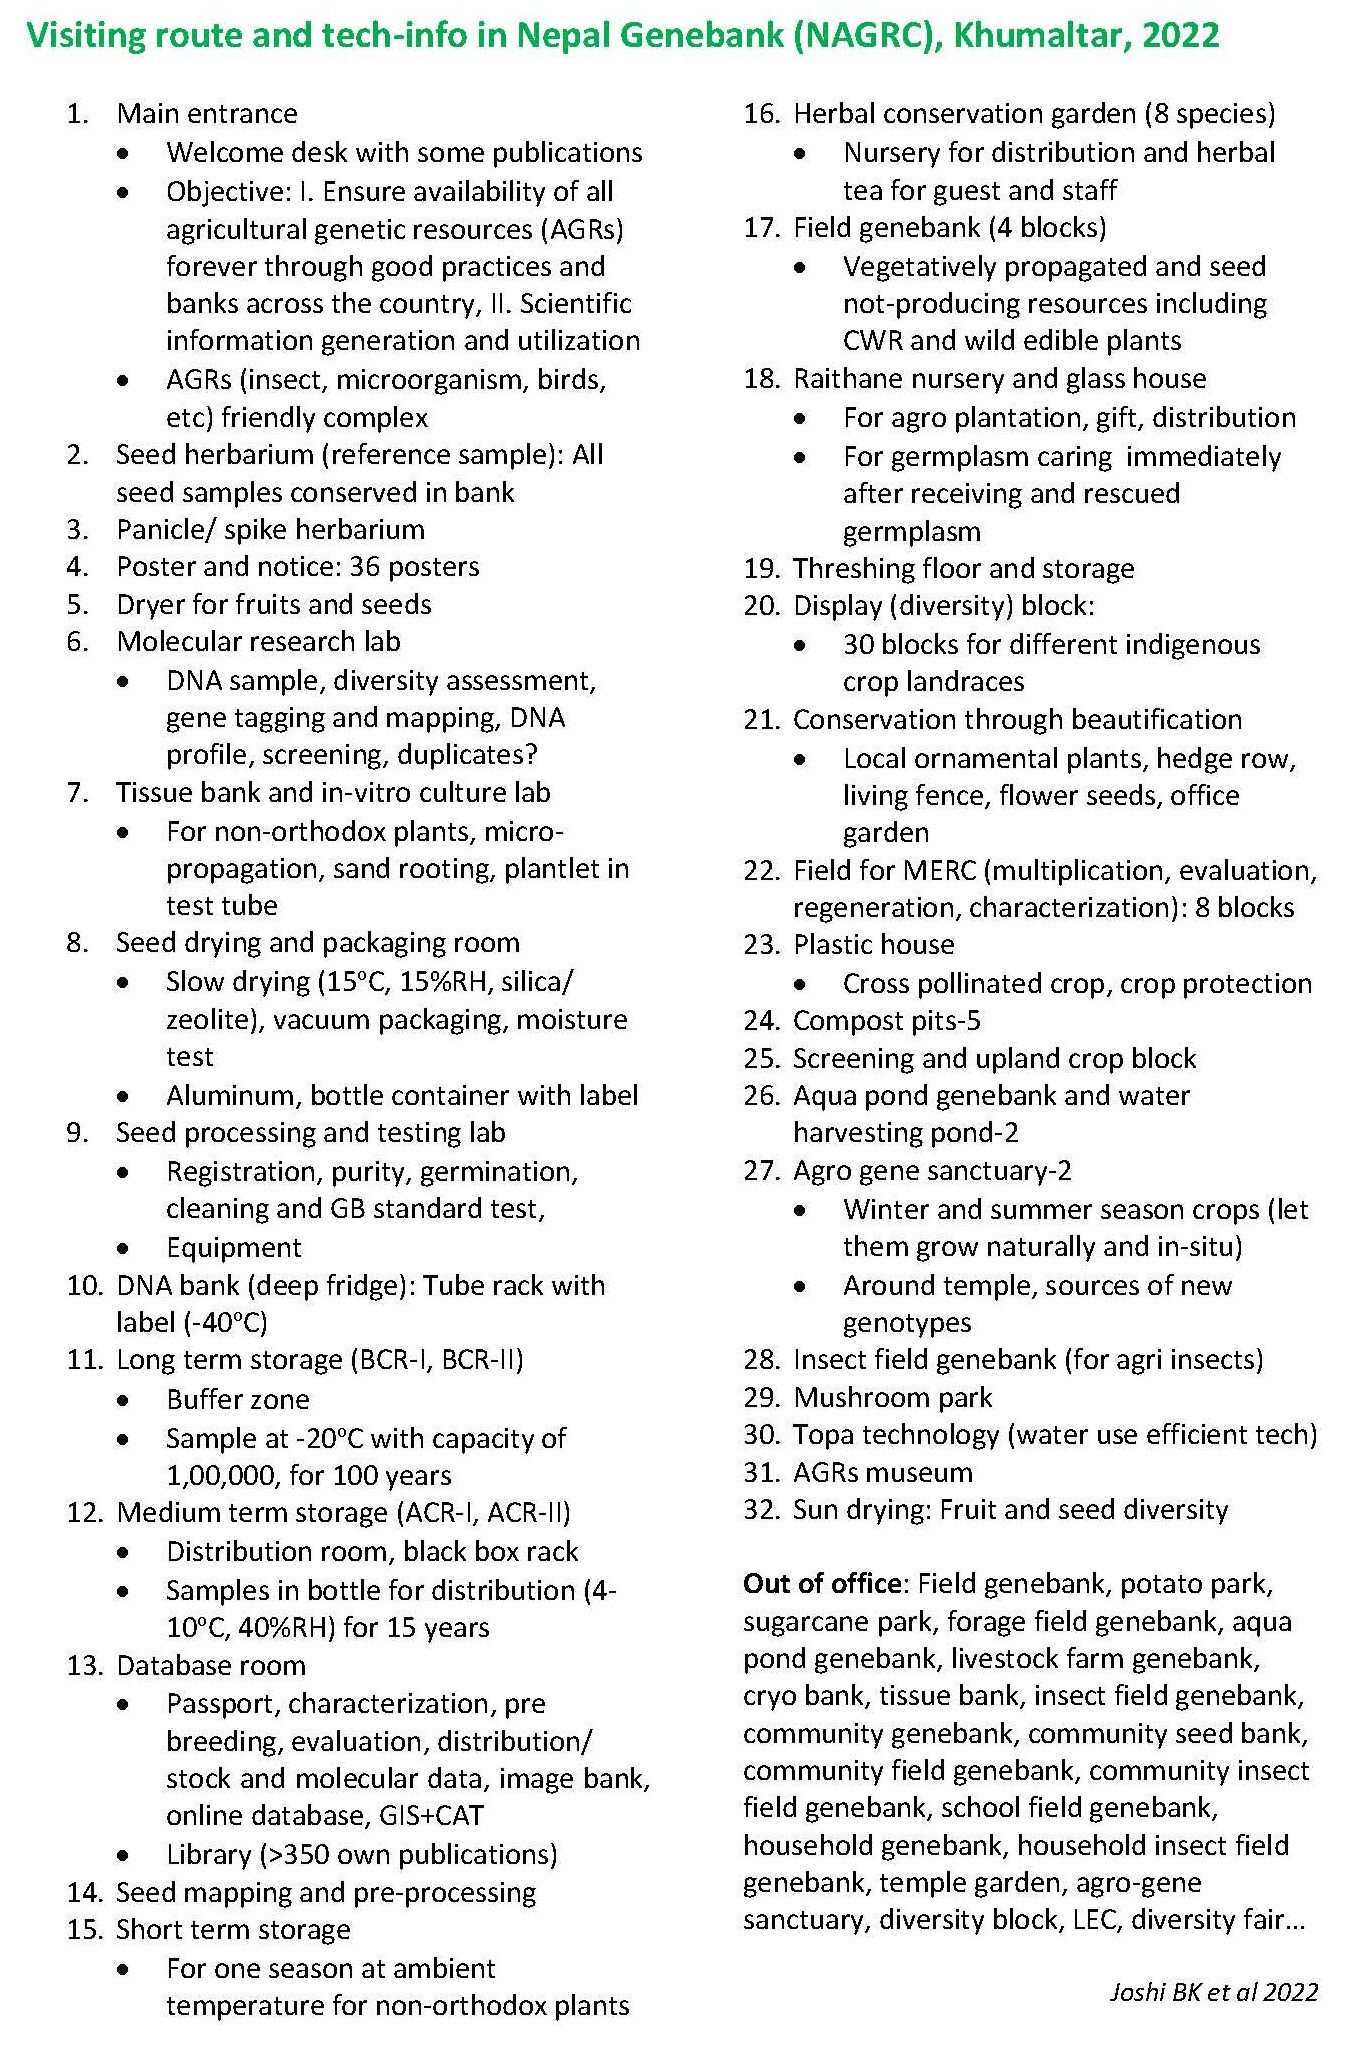
\includegraphics[width=0.35\linewidth]{./../images/genebank_nepal_components} \caption{Components of National Gene Bank, Khumaltar, Lalitpur}\label{fig:national-gene-bank}
\end{figure}
\end{frame}

\hypertarget{agrobiodiversity}{%
\section{Agrobiodiversity}\label{agrobiodiversity}}

\begin{frame}{Status in Nepal}
\protect\hypertarget{status-in-nepal}{}
\footnotesize

\begin{itemize}
\tightlist
\item
  Interplay of physical diversity and human management diversity gives
  rise to complexity in \textbf{agro-biodiversity}.
\end{itemize}

\begin{figure}
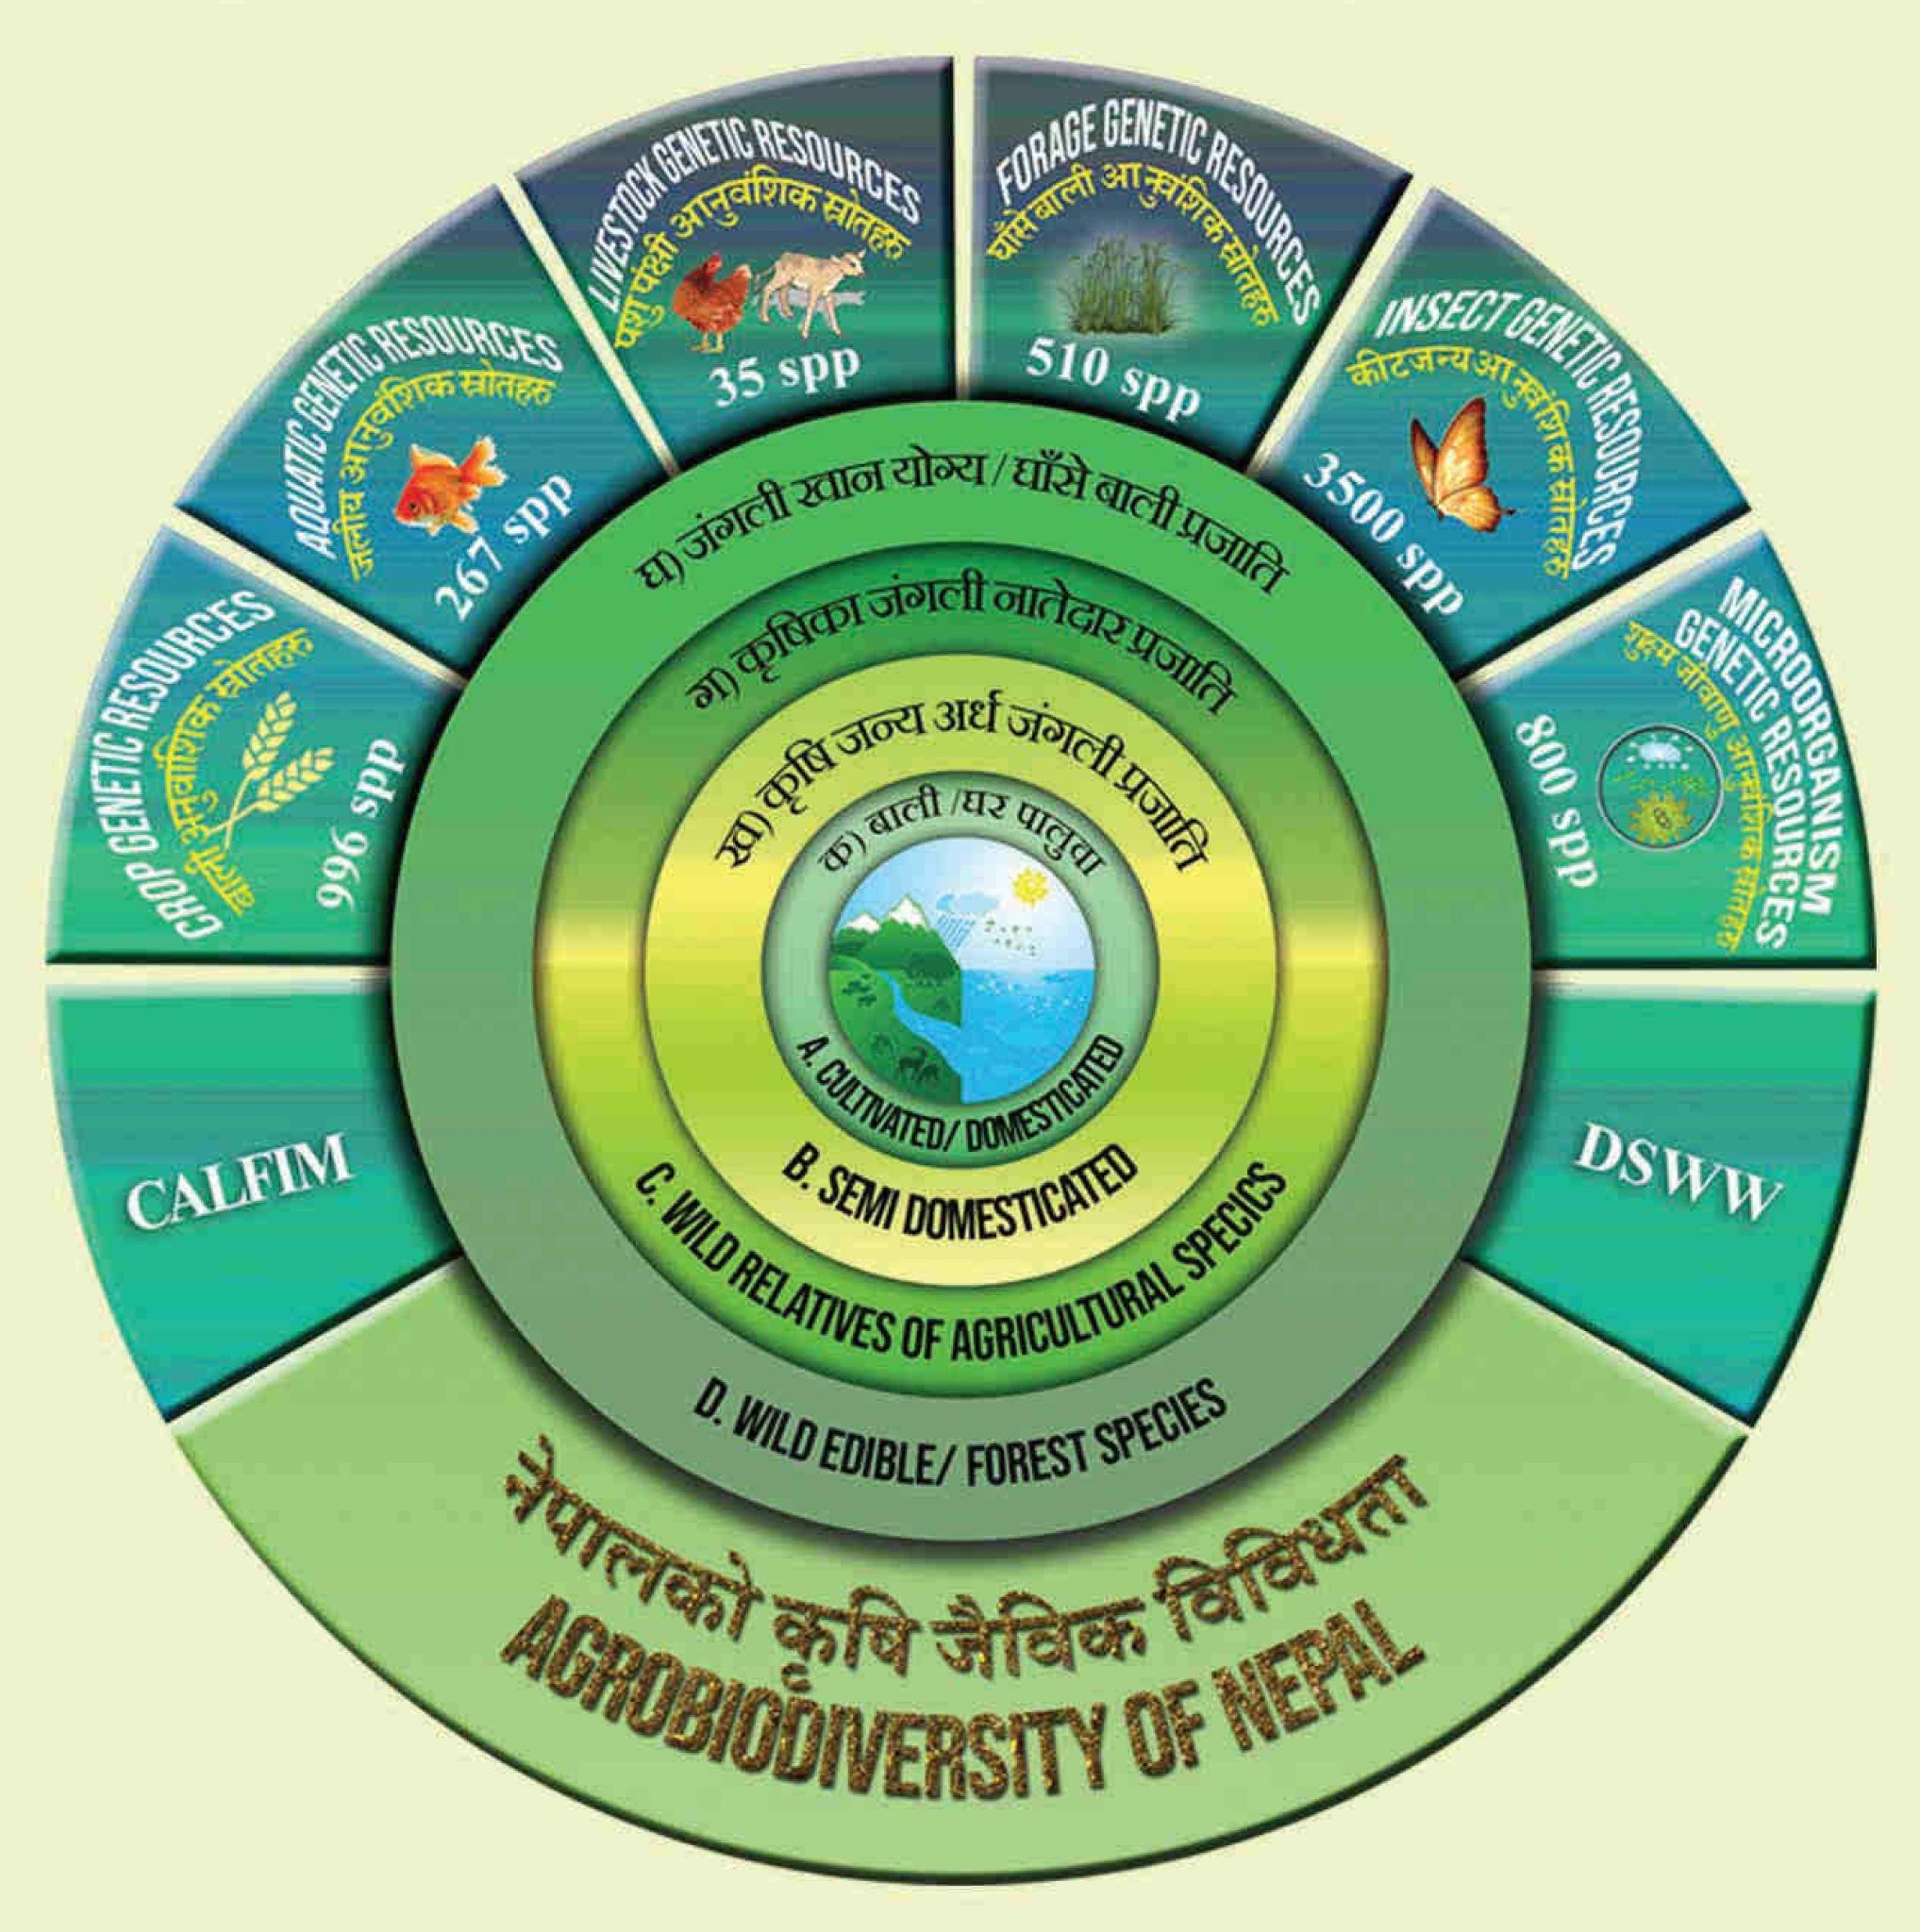
\includegraphics[width=0.38\linewidth]{./../images/agro_biodiversity_status_nepal} \caption{Agrobiodiversity status of Nepal, as assessed on 2022.}\label{fig:agrobiodiversity-status}
\end{figure}
\end{frame}

\begin{frame}{On farm conservation}
\protect\hypertarget{on-farm-conservation}{}
\begin{columns}[T,onlytextwidth]
  \column{0.4\textwidth}
  
  \begin{itemize}
  \footnotesize
  \item Agrobiodiversity largely entails on-farm conservation
  \item Its conservation objectives are met due to:
  \begin{itemize}
    \item Seed preservation by farmer household
    \item Participatory variety breeding
    \item Culture based importance for conservation
  \end{itemize}
  \end{itemize}

  \column{0.6\textwidth}
  
\begin{figure}
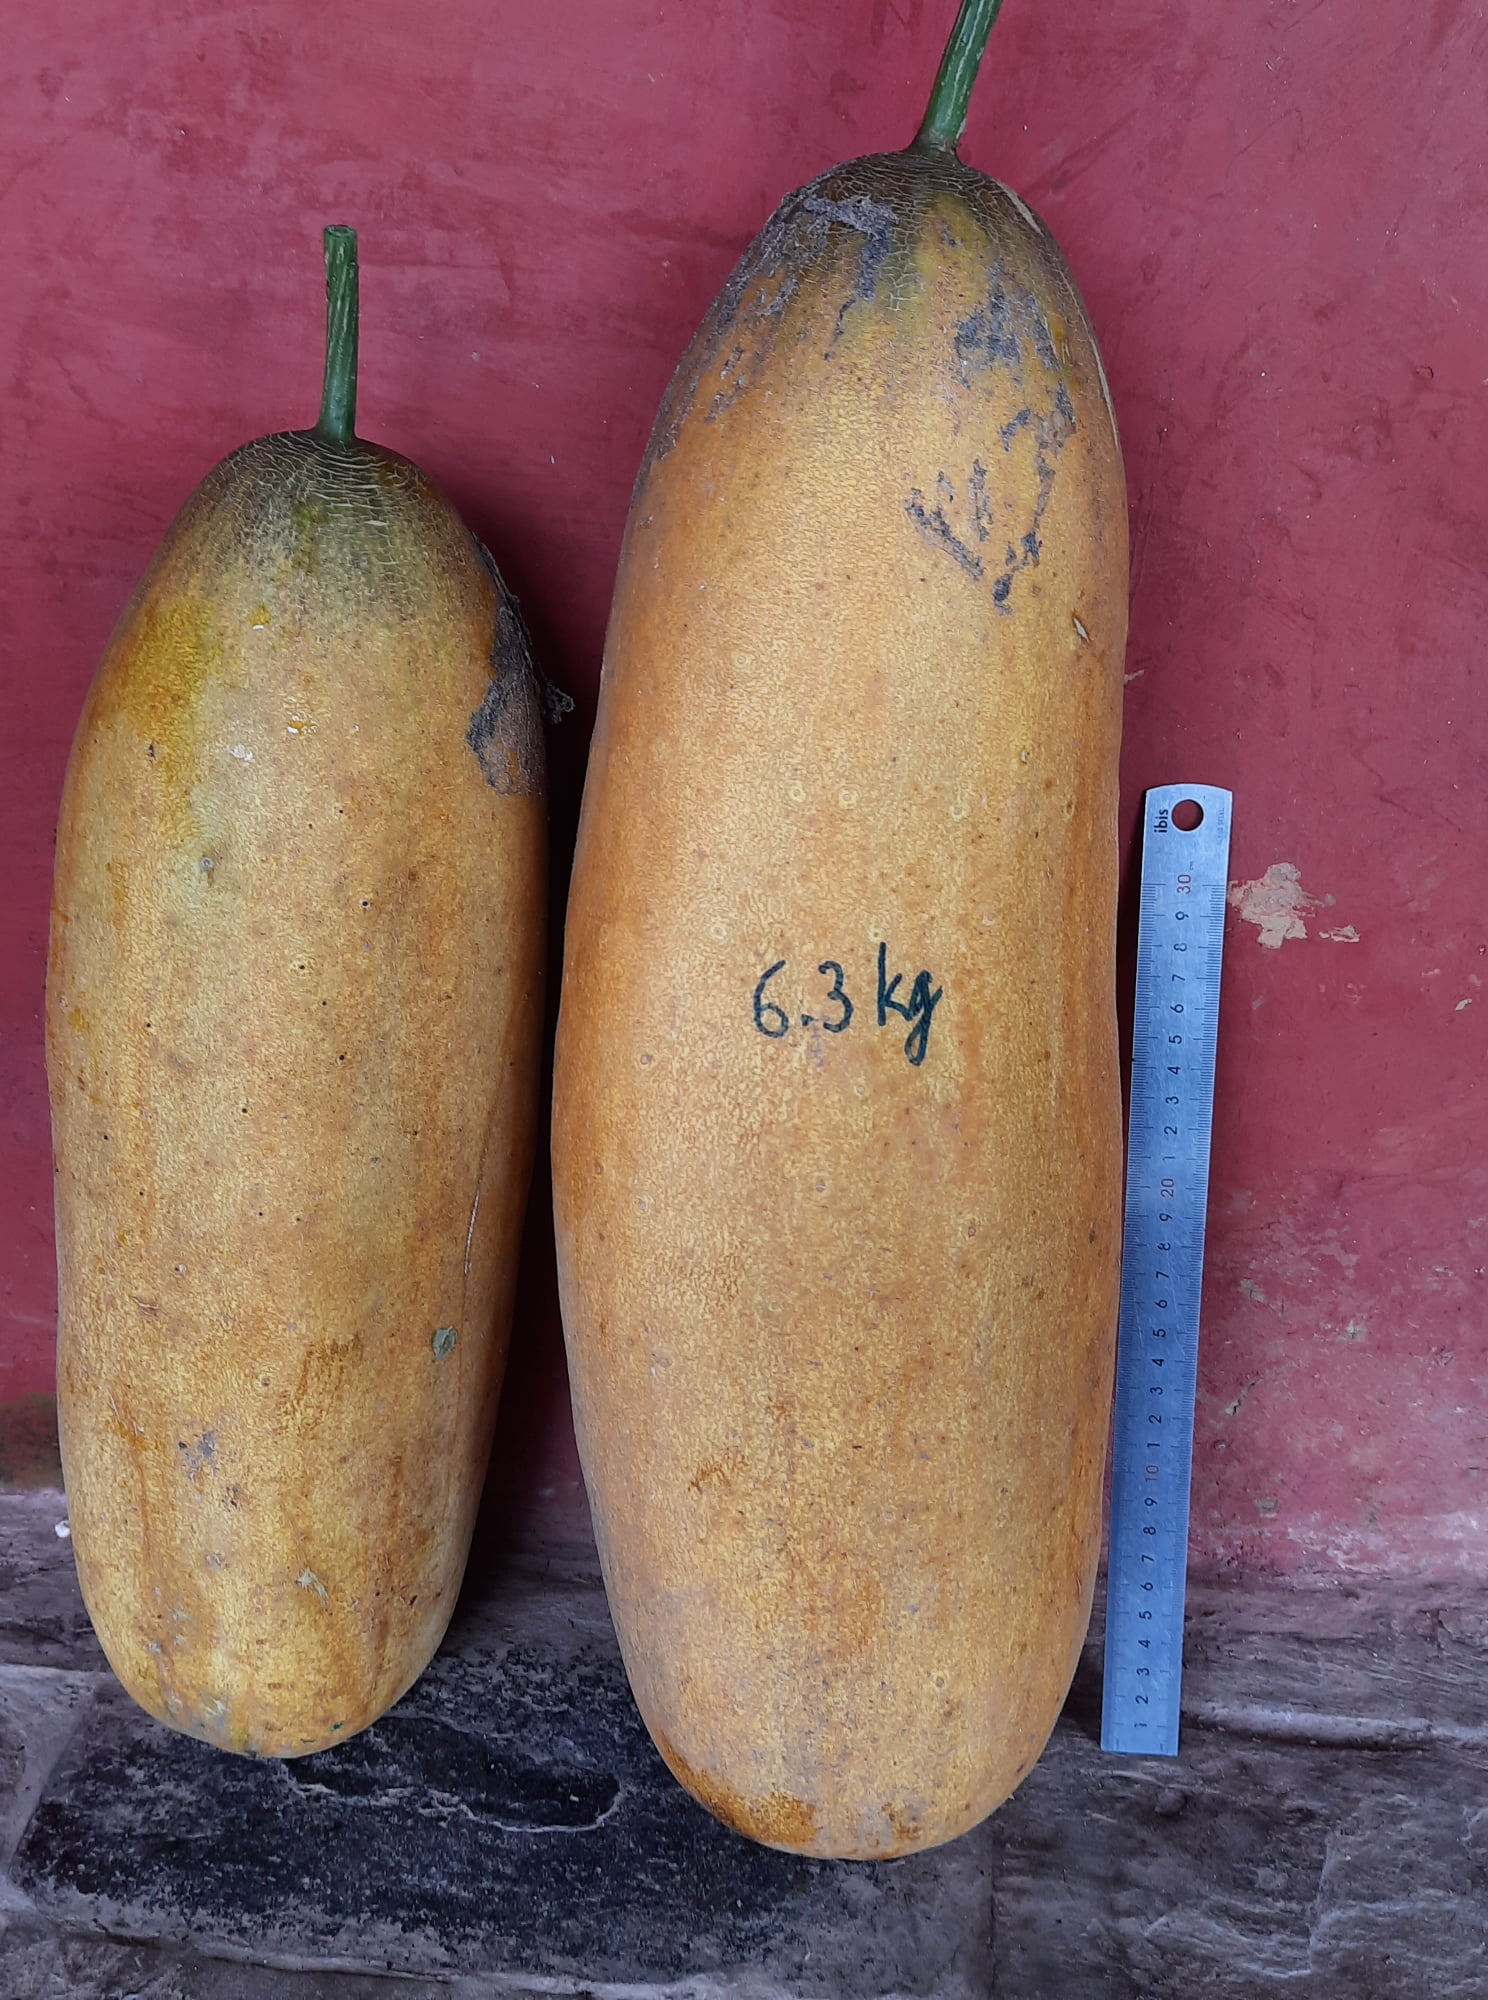
\includegraphics[width=0.55\linewidth]{./../images/madale_kakro} \caption{Participatory breeding of cucumber variety 'Madale' in Annapurna, Kaski.}\label{fig:participatory-breeding}
\end{figure}

\end{columns}
\end{frame}

\begin{frame}{Banking of Agricultural Genetic Resources}
\protect\hypertarget{banking-of-agricultural-genetic-resources}{}
\begin{itemize}
\tightlist
\item
  In academic institutions
\item
  In community based organizations
\item
  Field gene bank
\item
  Insect field gene bank -- Gabor valley gene bank (homestay), Banke
\item
  Aqua pond gene bank
\item
  Avian farm gene bank
\item
  Agro gene sanctuary
\end{itemize}
\end{frame}

\begin{frame}{Year of Agro-biodiversity}
\protect\hypertarget{year-of-agro-biodiversity}{}
\begin{figure}
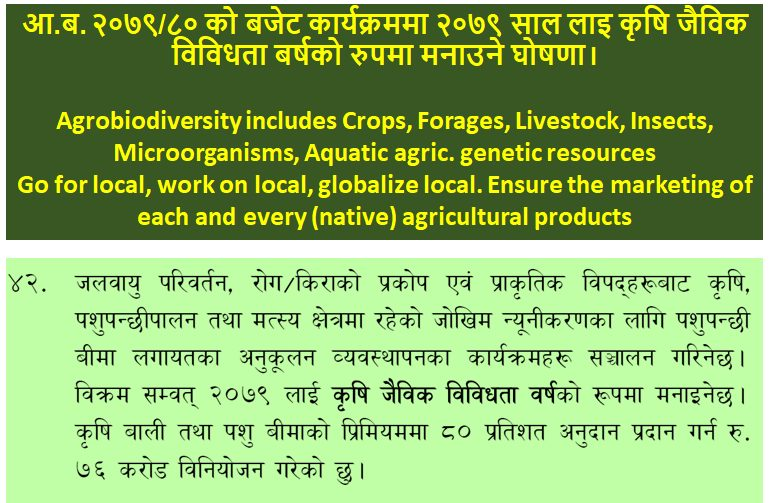
\includegraphics[width=0.7\linewidth]{./../images/budget_speech_year2078_79_of_agro_biodiversity} \caption{Budget speech of the FY 2078/79 declared the Year of Agrobiodiversity}\label{fig:year-of-agrobiodiversity207879}
\end{figure}
\end{frame}

\begin{frame}{Utilization of Agrobiodiversity resources}
\protect\hypertarget{utilization-of-agrobiodiversity-resources}{}
\begin{itemize}
\tightlist
\item
  Plant genetic resources: some new directions (Williams 1991)
\item
  Utilization of wild species for crop improvement (Stalker 1980)
\item
  Dynamic conservation of plant genetic resources (Bretting and Duvick
  1997)
\item
  Conservation and use or rice genetic resources (Chang, Adair, and
  Johnston 1982)
\item
  Wheat genetics resource center: The first 25 years (Gill et al. 2006)
\end{itemize}
\end{frame}

\hypertarget{protected-area-conservation}{%
\section{Protected area
conservation}\label{protected-area-conservation}}

\begin{frame}{History}
\protect\hypertarget{history}{}
\footnotesize

\begin{itemize}
\tightlist
\item
  As long as 2000 years ago ancient societies in Greece, Rome, Asia, and
  Africa are known to have set aside areas as sacred groves or sites,
  while european societies had hunting grounds for use of royalty and
  the wealthy.
\item
  First protected area of world: Yellowstone National Park (1872).
\item
  Until recently, the motivations have seldom been the protection of
  biodiversity \emph{per se}, and have usually been based on culturally
  valued aspects of biodiversity and the broader landscape, for example,
  charismatic megafauna, attractive habitats, important watersheds,
  recreational areas, or endangered species.
\item
  Multiple functions of protected areas:

  \begin{itemize}
  \tightlist
  \item
    Scientific research,
  \item
    Wilderness protection,
  \item
    Preservation of species and genetic diversity,
  \item
    Maintenance of environmental services,
  \item
    Protection of specific natural and cultural features,
  \item
    Tourism and recreation,
  \item
    Education,
  \item
    Sustainable use of resources from natural ecosystems, and
  \item
    Maintenance of cultural and traditional attributes
  \end{itemize}
\end{itemize}
\end{frame}

\begin{frame}{Components}
\protect\hypertarget{components}{}
\begin{block}{International Union for Conservation of Nature}
A clearly defined geographical space, recognized, dedicated and managed through legal or other effective means, to achieve the long-term conservation of nature with associated ecosystem services and cultural values.
\end{block}

\begin{itemize}
\tightlist
\item
  12.9\% (114,000 sites) of earth's land surface now occur under
  protected areas.
\end{itemize}
\end{frame}

\begin{frame}{IUCN categories of protected areas}
\protect\hypertarget{iucn-categories-of-protected-areas}{}
\begin{enumerate}
\tightlist
\item
\end{enumerate}

\begin{enumerate}
[(a)]
\tightlist
\item
  Strict Nature Reserves; Areas set aside to protect biodiversity and
  possibly geological features within strict control of visitation, use
  and impact.
\item
  Wilderness Areas; Largely unmodified or slightly modified area,
  retaining natural character without human habitation.
\end{enumerate}

\begin{enumerate}
\setcounter{enumi}{1}
\tightlist
\item
  National Parks; Natural or near natural areas to protect large scale
  ecological processes
\item
  Natural Monuments or Features; Landform, Sea mount, Submarine cavern,
  Cave, Living creature
\item
  Habitat/Species Management Areas; Particular species or habitats and
  management
\item
  Protected Landscape/Seascape: Area of interaction of people and nature
\item
  Protected area with sustainable use: Large area, low level industrial
  use of natural resource, with cultural associations for natural
  resource management.
\end{enumerate}
\end{frame}

\begin{frame}{Status of protected areas}
\protect\hypertarget{status-of-protected-areas}{}
\begin{figure}
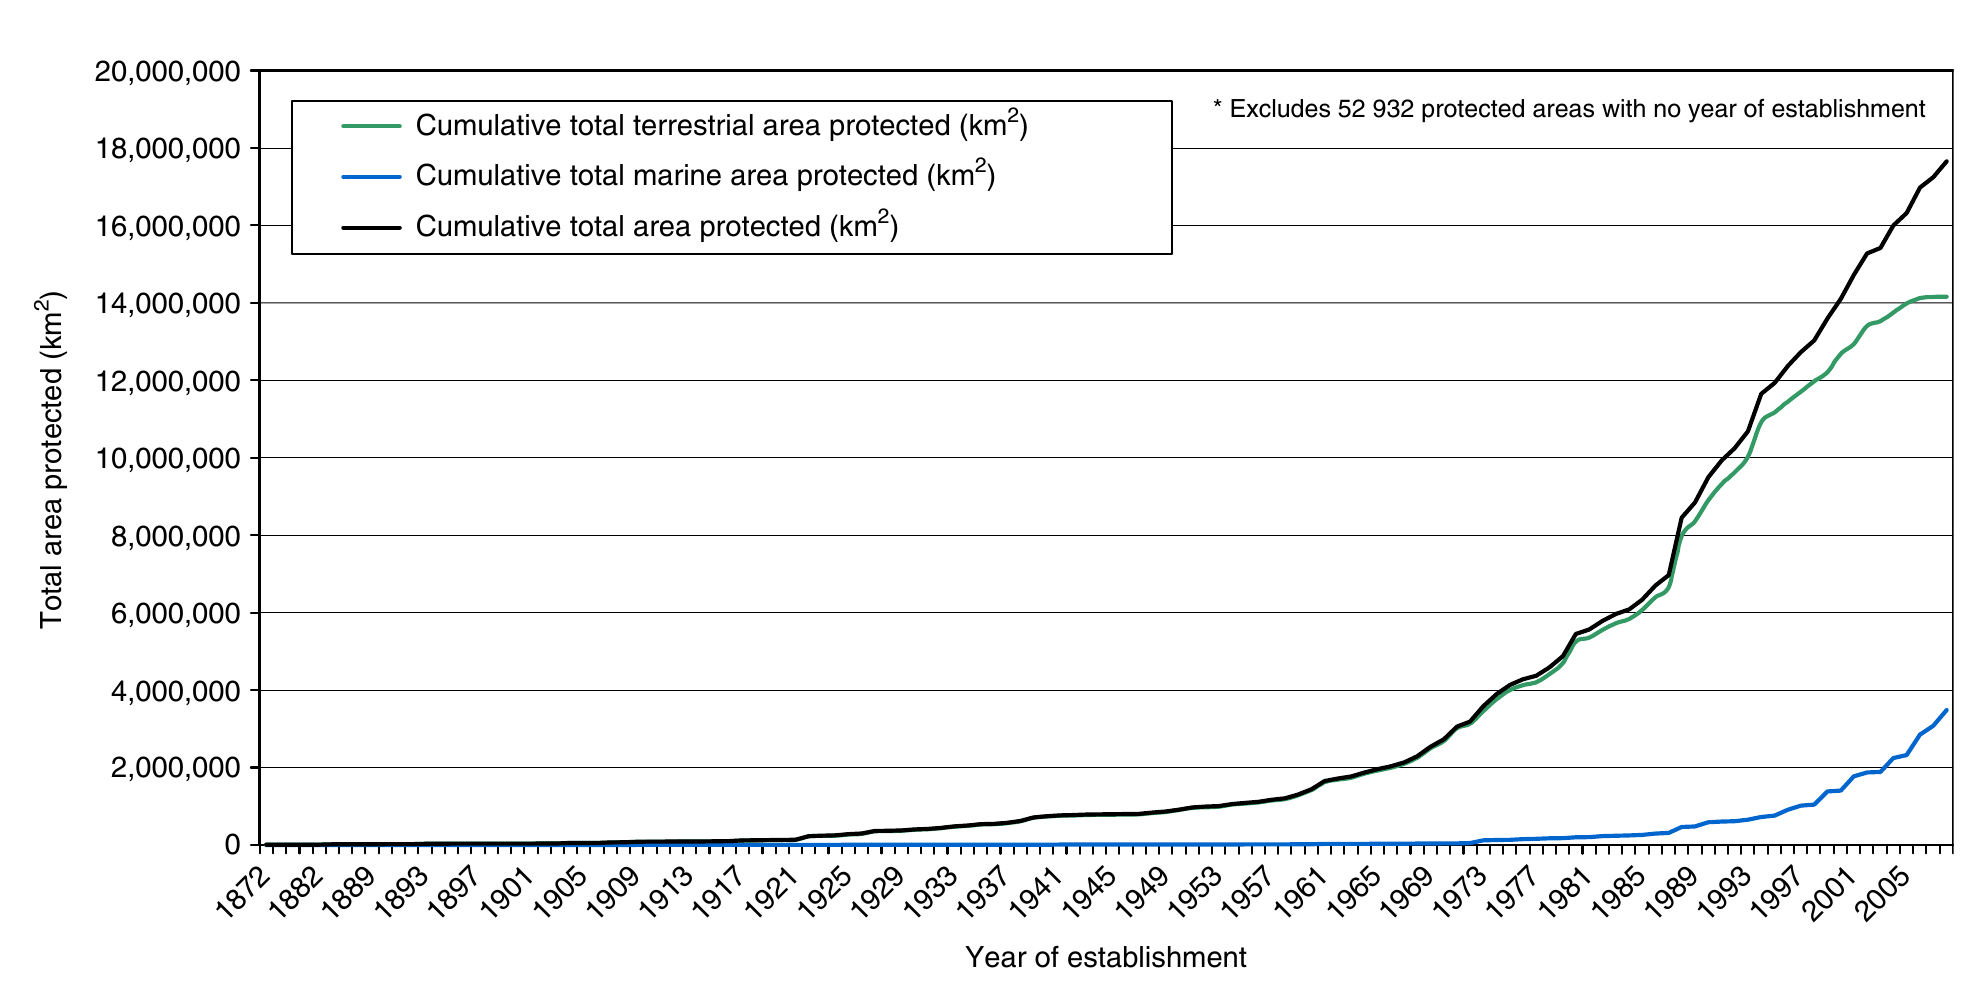
\includegraphics[width=0.65\linewidth]{./../images/global_protected_area} \caption{Global growth in protected areas. Reproduced from IUCN and UNEP-WCMC (2009).}\label{fig:global}
\end{figure}
\end{frame}

\begin{frame}{}
\protect\hypertarget{section-3}{}
\begin{figure}
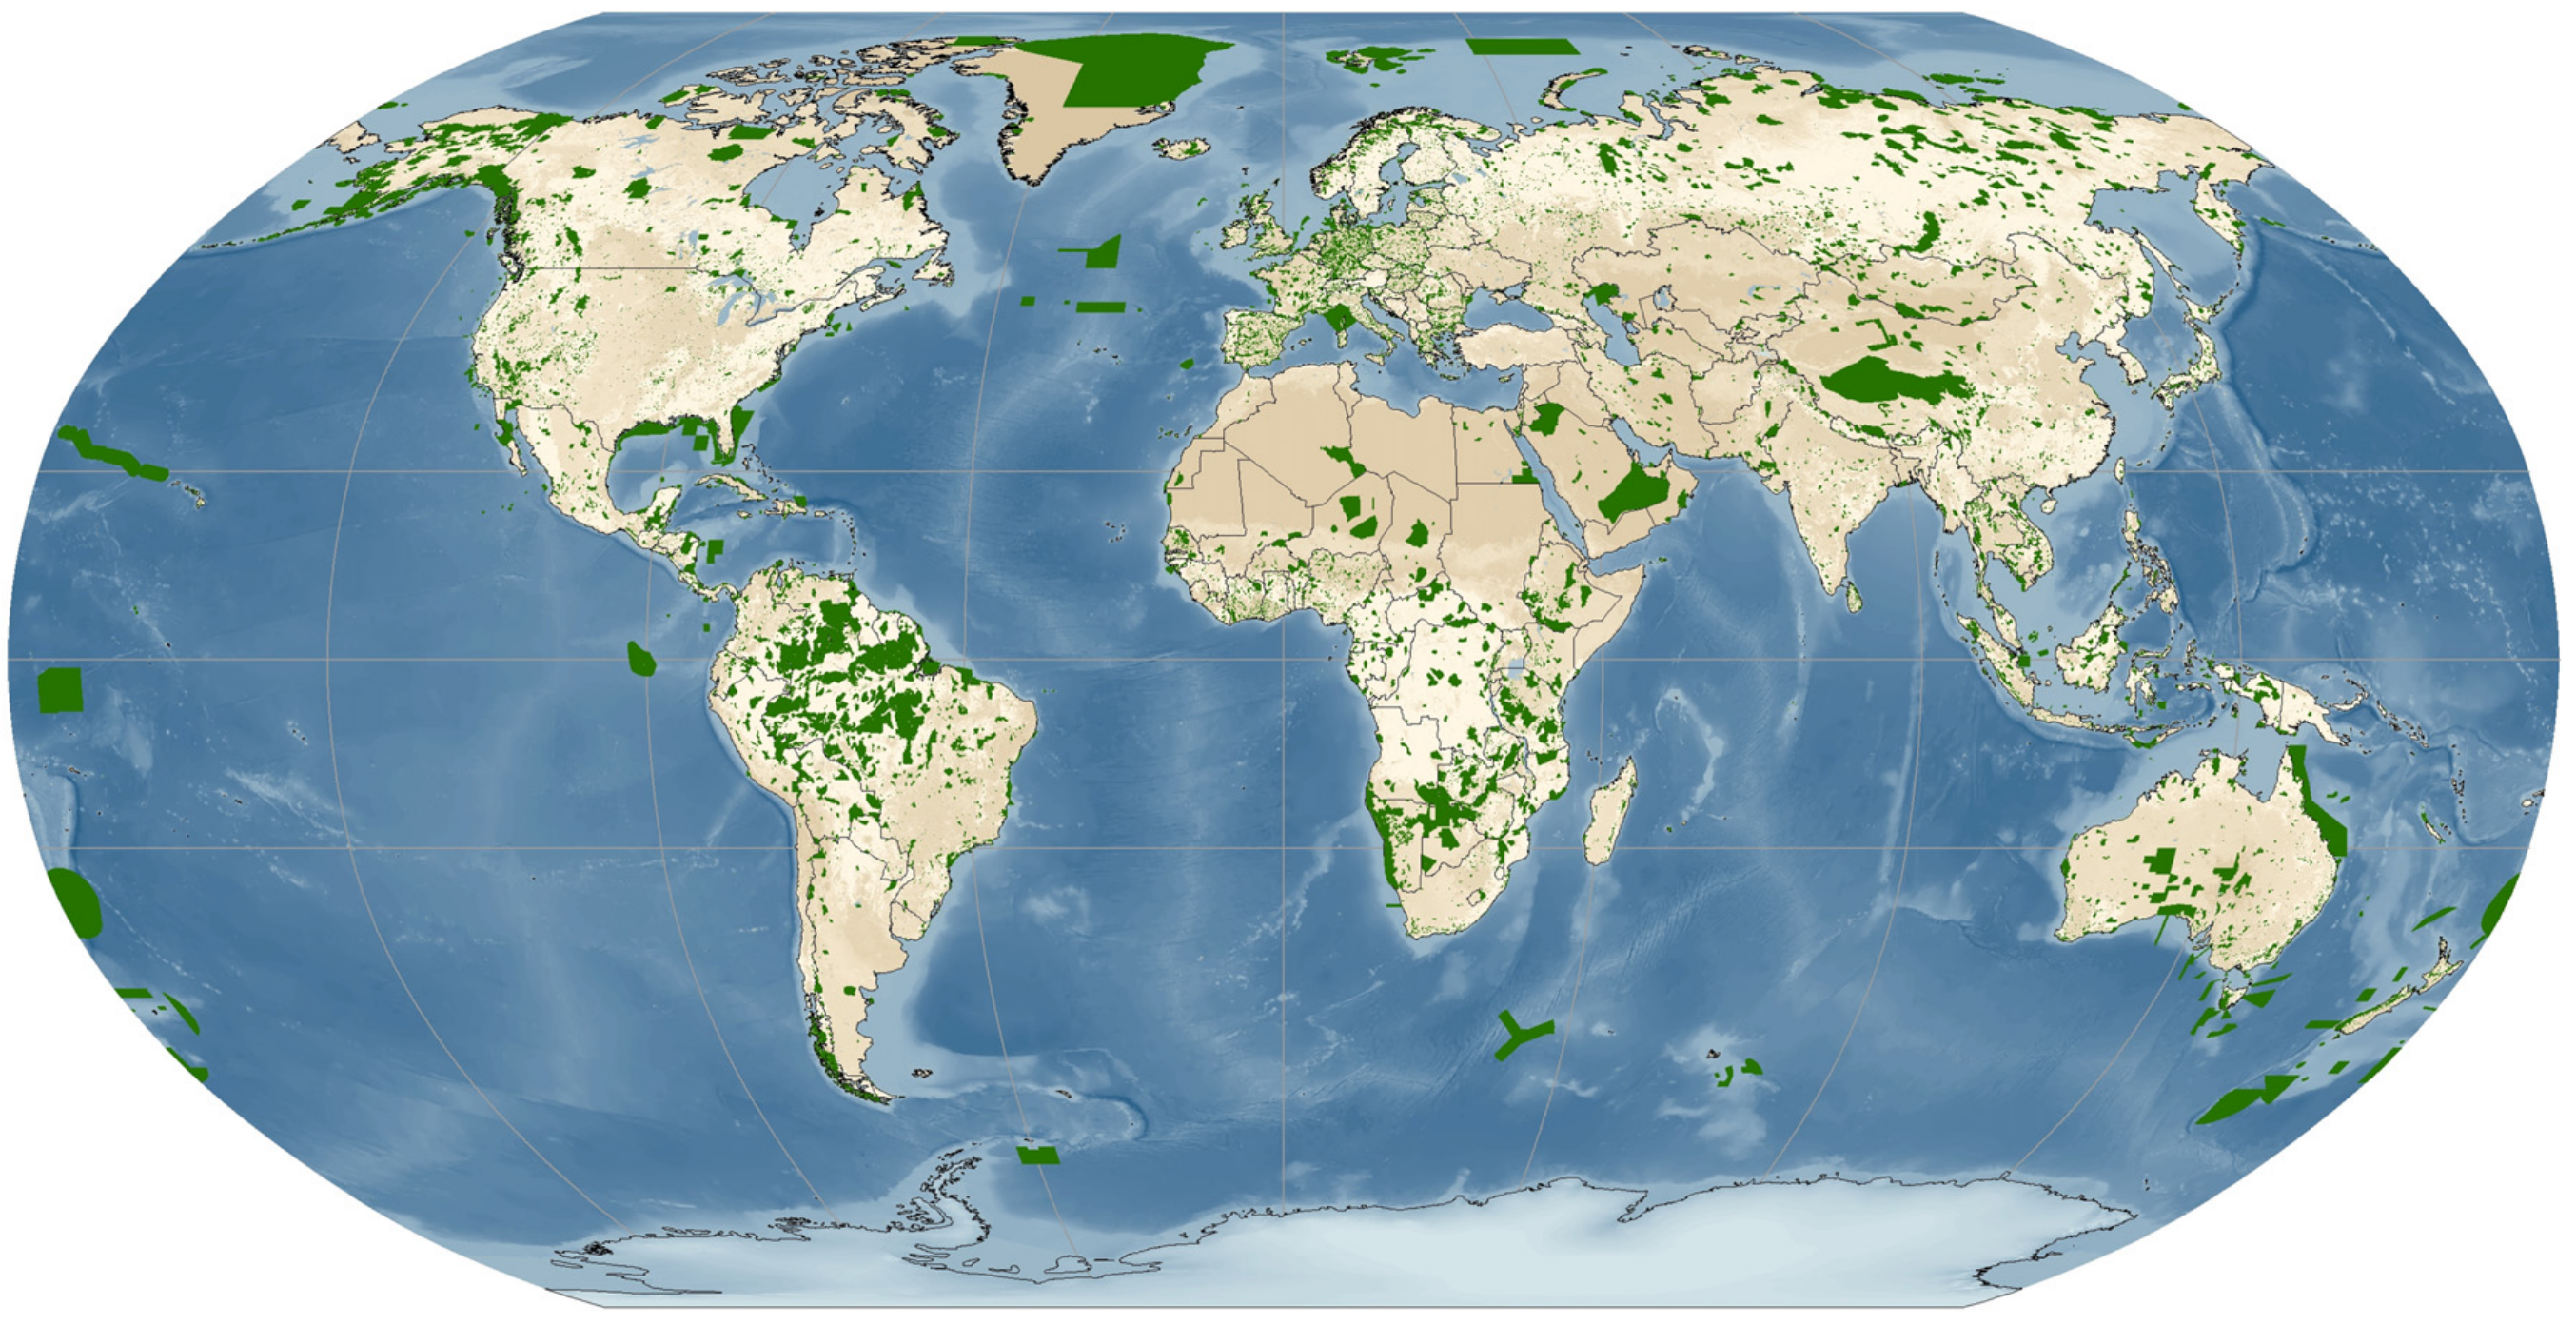
\includegraphics[width=0.8\linewidth]{./../images/global_protected_area_map} \caption{Protected areas of the world. Reproduced from World Database on Protected Areas (WDPA), UNEP-WCMC, July 2011.}\label{fig:global-map}
\end{figure}
\end{frame}

\begin{frame}{Protected area coverage of the world's biomes}
\protect\hypertarget{protected-area-coverage-of-the-worlds-biomes}{}
\begin{table}

\caption{\label{tab:unnamed-chunk-1}Protected area coverage of worlds biomes (in percentage)}
\centering
\fontsize{6}{8}\selectfont
\begin{tabular}[t]{lr}
\toprule
Biome & Percentage cover\\
\midrule
Tropical and subtropical moist broadleaf forests (TMF) & 5.5\\
Tropical and subtropical dry broadleaf forests (TDF) & 5.0\\
Tropical and subtropical coniferous forests (TCF) & 2.5\\
Temperate broadleaf and mixed forests (TeBF) & 3.8\\
Temperatre coniferous forests (TeCF) & 8.8\\
\addlinespace
Boreal forests/taiga (BF) & 6.2\\
Tropical and subtropical grasslands, savannas, and shrublands (TG) & 5.8\\
Temperate grasslands, savannas, and shrublands (TeG) & 2.0\\
Flooded grasslands and savannas (FG) & 8.8\\
Montane grasslands and shrublands (MG) & 3.8\\
\addlinespace
Tundra (T) & 13.8\\
Mediteranean forests, woodlands, and scrub or Sclerophyll forests (MF) & 3.0\\
Deserts and xeric shrublands (D) & 3.8\\
Mangrove (M) & 8.5\\
\bottomrule
\end{tabular}
\end{table}
\end{frame}

\begin{frame}{Protected areas in Nepal}
\protect\hypertarget{protected-areas-in-nepal}{}
\begin{itemize}
\tightlist
\item
  The country's protected area grew by more than 30 times in between
  1973 and 2010.
\item
  Currently, 23.23 percent of the country's total land area is under
  protection (one of the highest in Asia).
\item
  Populations of some flagship species, including tiger and rhino, have
  increased in recent years.
\item
  Efforts have been made to link local communities to benefits of
  protected areas through the establishment and management of
  conservation areas and buffer zones.
\end{itemize}
\end{frame}

\begin{frame}{}
\protect\hypertarget{section-4}{}
\begin{table}
\centering\begingroup\fontsize{5}{7}\selectfont

\begin{tabular}{>{\raggedright\arraybackslash}p{8em}>{\raggedright\arraybackslash}p{4em}>{\raggedright\arraybackslash}p{3em}>{\raggedright\arraybackslash}p{5em}>{\raggedright\arraybackslash}p{48em}}
\toprule
Protected Area & Year Established & Area (sq. km.) & Elevation (m) & Conservation Significance\\
\midrule
\textbf{\cellcolor{gray!6}{1 Chitwan (World Heritage Site 1984)}} & \cellcolor{gray!6}{1973} & \cellcolor{gray!6}{932} & \cellcolor{gray!6}{150-815} & \cellcolor{gray!6}{The Park houses over 50 species of mammals including one-horned rhinoceros, Royal Bengal tiger and bison; Important Bird Area; 539 species of birds that include migrant birds like paradise flycatcher, Indian pitta, parakeets and several species of waterfowl; and many species of amphibians and reptiles including the endangered gharial, marsh mugger crocodile and python. The habitat comprises of deciduous broadleaf forest with over 600 plant species, savannas and wetlands.}\\
\textbf{2 Langtang} & 1976 & 1710 & 792-7,245 & The habitat types range from sub-tropical forests below 1,000 m to alpine shrubs and grasslands. Musk deer and red panda are at the focus of conservation. Many other mammals such as snow leopard, wild dog, Himalayan black bear, Himalayan tahr, ghoral, serow, rhesus monkey and langur monkey, and over 370 species of birds including tragopan and impeyan pheasant (danphe) are found.\\
\textbf{\cellcolor{gray!6}{3 Rara}} & \cellcolor{gray!6}{1976} & \cellcolor{gray!6}{106} & \cellcolor{gray!6}{1,800-4,048} & \cellcolor{gray!6}{Rara has many animal species including endangered red panda and musk deer. Three species of snow trout are found in the lake. During winter over 270 species of birds including coots, great-crested grebe, black-necked grebe, red crested pochard, mallard, common teal, merganser and gulls, and migrant water fowls can be seen. Coniferous forests, primarily of blue pine forms the dominant vegetation. Rhododendron, juniper, spruce, oak and cypress are found around 3,000 m while spruce and fir are more common at higher elevations.}\\
\textbf{4 Sagarmatha (World Heritage Site 1979)} & 1976 & 1148 & 2,800-8,848 & The Park is famous for the scenic beauty of the Himalayas (including Mount Everest), musk deer, red panda, beer and snow leopard. Nearly 200 species of birds including impeyan pheasant, blood pheasant, red-billed chough, yellow-billed chough, snow cock, and snow pigeon are found. The forest vegetation comprises of pine and hemlock forests at lower elevations, and silver fir, birch, rhododendron and juniper at higher elevations (i.e. above 3,500 m).\\
\textbf{\cellcolor{gray!6}{5 Shey-Phoksundo}} & \cellcolor{gray!6}{1984} & \cellcolor{gray!6}{3555} & \cellcolor{gray!6}{2,000-6,885} & \cellcolor{gray!6}{Wild goat (ghoral), blue sheep, musk deer, and the Shey-Phoksundo lake are some of the main attractions. Over 200 species of birds including yellow throated marten, Tibetan partridge, wood snipe, white-throated tit, wood accentor and crimson-eared rose finch, impeyan pheasant, cheer pheasant, chough, raven, Tibetan snow cock, Tibetan twit and Himalayan griffon; and 29 species of butterflies are found. Pine, walnut, willow, oak, cypress are dominant trees in the lower elevations and pine, spruce, juniper and birch at higher elevations. Alpine range is comprised of meadows and shrubs of berberis, wild rose and caragana.}\\
\bottomrule
\end{tabular}
\endgroup{}
\end{table}
\end{frame}

\begin{frame}{}
\protect\hypertarget{section-5}{}
\begin{table}
\centering\begingroup\fontsize{5}{7}\selectfont

\begin{tabular}{>{\raggedright\arraybackslash}p{8em}>{\raggedright\arraybackslash}p{5em}>{\raggedright\arraybackslash}p{5em}>{\raggedright\arraybackslash}p{6em}>{\raggedright\arraybackslash}p{40em}}
\toprule
Protected Area & Year Established & Area (sq. km.) & Elevation (m) & Conservation Significance\\
\midrule
\textbf{\cellcolor{gray!6}{6 Khaptad}} & \cellcolor{gray!6}{1984} & \cellcolor{gray!6}{225} & \cellcolor{gray!6}{1,000-3,276} & \cellcolor{gray!6}{The Park is famous for medicinal plants. Over 220 species of medicinal plants are recorded. Wildlife includes barking deer, wild boar, ghoral, Himalayan black bear, yellow-throated marten, rhesus monkey and langur monkey, and around 270 species of birds are found. Vegetation is mainly comprised of grasslands and subtropical, temperate, and sub alpine forests. This is also a famous spiritual site}\\
\textbf{7 Bardia} & 1988 & 968 & 152-1,494 & Mammals such as Royal Bengal tiger, one-horned rhinoceros, elephant, swamp deer, black buck, and reptiles such as gharial, marsh mugger crocodile are the main species. Fresh-water Gangetic dolphin is found in the Karnali River. Bengal florican, lesser florican, silver-eared mesia and sarus crane are some of 400 species of birds found in the Park that is dominated by sal forest and savannahs.\\
\textbf{\cellcolor{gray!6}{8 Makalu Barun}} & \cellcolor{gray!6}{1991} & \cellcolor{gray!6}{1500} & \cellcolor{gray!6}{435-8,463} & \cellcolor{gray!6}{The park is an important habitat for endangered red panda and snow leopard, and several species of endangered plants. Above 80 varieties of fish including salmon are reported in the Arun River. Wren babbler and olive ground warbler are some of the 400 species of birds found in the Park. Forest vegetation ranges from sub-tropical forests to sub-alpine and alpine vegetation as the elevation increases. The park is also famous for Rhododendrons and orchids.Twenty-five (out of 30 found in Nepal) varieties of rhododendrons, 48 species of orchids, 87 species of medicinal herbs, 48 species o primroses and 86 species of fodder trees are reportedly found in the Park.}\\
\textbf{9 Shivapuri-Nagarjun} & 2002 & 159 & 1,366-2,732 & Conservation of watershed that drains the Kathmandu Valley is a major objective. Around 19 species of mammals including Himalayan black bear, leopard, barking deer, wild boar, wild cat, rhesus monkey and langur monkey, 177 species of birds, 102 species of butterflies, and 129 varieties of mushrooms are reported.\\
\textbf{\cellcolor{gray!6}{10 Banke}} & \cellcolor{gray!6}{2010} & \cellcolor{gray!6}{550} & \cellcolor{gray!6}{360-480} & \cellcolor{gray!6}{Conservation of endangered wildlife and strengthening of transboundary biological corridor are some of the main objectives. Includes eight natural ecosystems, and houses 124 species of plants, 34 mammals, more than 300 birds, 24 reptiles, seven amphibians, and 58 fish species}\\
\bottomrule
\end{tabular}
\endgroup{}
\end{table}
\end{frame}

\begin{frame}{}
\protect\hypertarget{section-6}{}
\begin{table}
\centering\begingroup\fontsize{5}{7}\selectfont

\begin{tabular}{>{\raggedright\arraybackslash}p{8em}>{\raggedright\arraybackslash}p{5em}>{\raggedright\arraybackslash}p{5em}>{\raggedright\arraybackslash}p{6em}>{\raggedright\arraybackslash}p{40em}}
\toprule
Protected Area & Year Established & Area (sq. km.) & Elevation (m) & Conservation Significance\\
\midrule
\textbf{\cellcolor{gray!6}{1 Shuklaphanta}} & \cellcolor{gray!6}{1976} & \cellcolor{gray!6}{305} & \cellcolor{gray!6}{90-270} & \cellcolor{gray!6}{Major wildlife consists of swamp deer, wild elephant, tiger, several species of deer, wild boar, leopard, and monkeys. Marsh mugger crocodile, cobra, and python are Common reptiles.Important Bird Area; Saruscrane,swampfrancolin,grassowl, warblers, flycatchers, Bengal florican are the common birds found in the sub-tropical sal forest and open grasslands.}\\
\textbf{2 Koshi Tappu (Ramsar Site, 1987)} & 1976 & 175 & 80-100 & Wild buffalo and Siberian migratory birds are the main focus of conservation. Vegetation consists of grasslands with patches of scrub and deciduous riverine forests. Many other species of mammals (such as wild elephants, wild boar, hog deer, spotted deer, blue bull and jackal); Important Bird Area; 479 species of birds, and reptiles are found. Gangetic dolphins are found in the Koshi River.\\
\textbf{\cellcolor{gray!6}{3 Parsa}} & \cellcolor{gray!6}{1984} & \cellcolor{gray!6}{499} & \cellcolor{gray!6}{150-815} & \cellcolor{gray!6}{Wildlife species including wild elephant, tiger leopard, sloth bear, and gaur; reptiles including king cobra, common cobra, krait, rat snake and python; over 370 species of birds including the endangered great hornbill are reported. Natural vegetation consists of tropical and sub-tropical sal forests. Chir pine, khair, and sissoo trees are found on the hilly parts.}\\
\textbf{1 Dhorpatan} & 1987 & 1325 & 2,850-7,000 & The reserve is famous for blue sheep, which is open for regulated trophy hunting\\
\textbf{\cellcolor{gray!6}{1 Annapurna}} & \cellcolor{gray!6}{1992} & \cellcolor{gray!6}{7629} & \cellcolor{gray!6}{1,000-8,092} & \cellcolor{gray!6}{Endemic plants and mountains are the main characteristics. Over 100 species of mammals including blue sheep and endangered snow leopard; 39 species of reptiles; 22 species of amphibians; Important Bird Area (IBA); 474 species of birds including multi-colored impeyan pheasant, kokla and blood pheasant are reported. Many species of orchids and rhododendrons are found.}\\
\bottomrule
\end{tabular}
\endgroup{}
\end{table}
\end{frame}

\begin{frame}{}
\protect\hypertarget{section-7}{}
\begin{table}
\centering\begingroup\fontsize{5}{7}\selectfont

\begin{tabular}{>{\raggedright\arraybackslash}p{8em}>{\raggedright\arraybackslash}p{5em}>{\raggedright\arraybackslash}p{5em}>{\raggedright\arraybackslash}p{6em}>{\raggedright\arraybackslash}p{40em}}
\toprule
Protected Area & Year Established & Area (sq. km.) & Elevation (m) & Conservation Significance\\
\midrule
\textbf{\cellcolor{gray!6}{2 Kanchanjunga}} & \cellcolor{gray!6}{1997} & \cellcolor{gray!6}{2035} & \cellcolor{gray!6}{1,200-8,598} & \cellcolor{gray!6}{Mammals including endangered snow leopard, Himalayan black bear, musk deer, red panda, blue sheep, rhesus monkey; 252 species of different birds including impeyan pheasant, red-billed blue magpie, ashy drongo; 20 indigenous gymnosperms, 15 among Nepal's 23 endemic flowering plants, 30 varieties of rhododendrons and 48 varieties of orchids are reported.}\\
\textbf{3 Manasula} & 1998 & 1663 & 1,360-8,163 & Snow leopard, musk deer and Himalayan Tahr are among the 33 species of mammals found in the conservation area. Over 110 species of birds and 1,500-2,000 species of flowering plants are reported.\\
\textbf{\cellcolor{gray!6}{5 Khairapur}} & \cellcolor{gray!6}{2010} & \cellcolor{gray!6}{16} & \cellcolor{gray!6}{120-230} & \cellcolor{gray!6}{The first organized effort to conserve the endangered blackbuck (Antilope cervicapra).}\\
\textbf{6 Api Nampa} & 2010 & 1903 & 539-7,132 & Snow leopard, musk deer, clouded leopard, ghoral, Himalayan black bear and Himalayan tahr are found in the area.\\
\bottomrule
\end{tabular}
\endgroup{}
\end{table}
\end{frame}

\begin{frame}{Framework for reviewing contribution}
\protect\hypertarget{framework-for-reviewing-contribution}{}
\begin{figure}
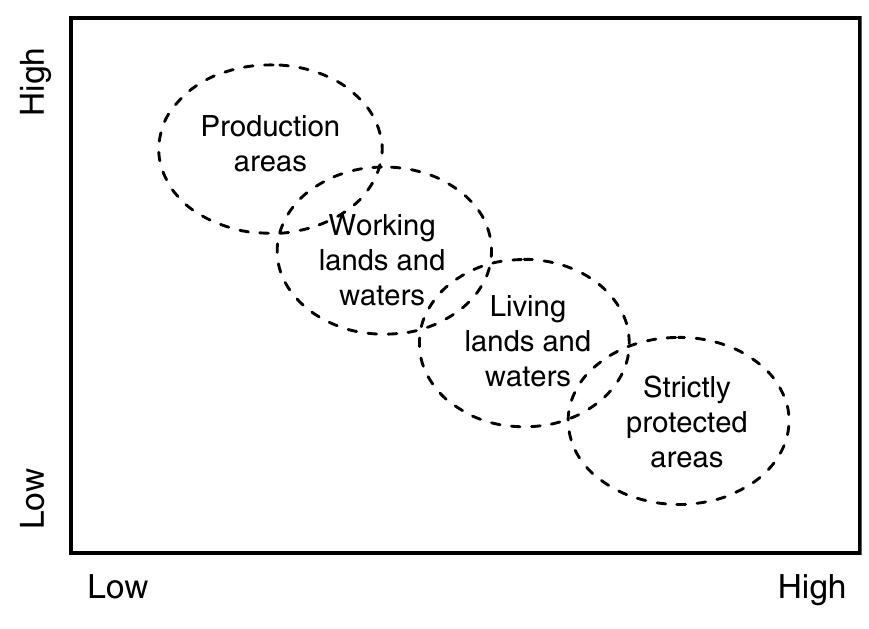
\includegraphics[width=0.45\linewidth]{./../images/contribution_review} \caption{A framework for reviewing the contribution of areas of land and water to biodiversity conservation. Starting at the bottom right hand corner the framework moves from 'strictly protected areas', reflecting the more traditional approach to protected areas managed almost exclusively for biodiversity conservation, The next category is 'living lands and waters', which are areas managed primarily for biodiversity conservation with some extractive uses limited to the ecologically sustainable management of areas of land and water to support life of all forms. 'Working lands and waters' are mostly agricultural lands managed primarily for extractive uses while attempting to conserve biodiversity at the same time. The final category is 'production areas' of land and water where the management focuses exclusively on maximizing extractive and productive uses and biodiversity conservation is not an objective.}\label{fig:contribution-review}
\end{figure}
\end{frame}

\hypertarget{national-legislation-on-biodiversity}{%
\section{National legislation on
biodiversity}\label{national-legislation-on-biodiversity}}

\begin{frame}{National biodiversity strategy and action plan}
\protect\hypertarget{national-biodiversity-strategy-and-action-plan}{}
\begin{itemize}
\tightlist
\item
  GoN prepared and implemented National Biodiversity Strategy (NBS) in
  2002 and Nepal Biodiversity Strategy Implementation Plan in 2006.
\item
  Ministry of Forest and Soil Conservation (MoFSC) revised the earlier
  documents into National Biodiversity Strategy and Action Plan (NBSAP,
  2014-2020) with support from Global Environmental Facility through
  United National Environment Programme (UNEP).
\item
  The CBD's Strategic Plan for Biodiversity 2011--2020 and the Aichi
  Biodiversity Targets provided theoretical framework and technical
  guidance in its development.
\item
  Provides long term (35 years) and short term (upto 2020) strategies
  and priorities
\end{itemize}
\end{frame}

\begin{frame}{}
\protect\hypertarget{section-8}{}
\footnotesize

\begin{itemize}
\tightlist
\item
  Description and analysis of past efforts and achievements, and
  formulation of strategies and actions are focused around 6 thematic
  areas:

  \begin{itemize}
  \tightlist
  \item
    Protected areas
  \item
    Forests outside protected areas
  \item
    Rangelands
  \item
    Wetlands
  \item
    Agriculture
  \item
    Mountains
  \end{itemize}
\item
  Quantitative targets have been set against each priority action, where
  appropriate.
\item
  The framework for Local Biodiversity Strategy and Action Plan
  highlights key aspects of biodiversity management at local (VDC and
  Municipality) level, intended to serve as guide in preparing their own
  strategy and action plan.
\end{itemize}
\end{frame}

\begin{frame}{}
\protect\hypertarget{section-9}{}
\begin{itemize}
\tightlist
\item
  The NBSAP provides a reference status of biodiversity in Nepal. (For
  the exact account, refer to lecture slides on ``Biodiversity: Concept,
  Aim and Scope'').
\item
  It suggests local, institutional and sectoral/thematic and
  cross-sectora/thematic strategies for biodiversity management
  (discussed below).
\item
  Other policy papers forming guidelines in biodiversity management
  include:

  \begin{itemize}
  \tightlist
  \item
    The Herbs and Non-Timber Forest Products Development Policy (2004),
  \item
    Agrobiodiversity Policy (2007),
  \item
    Tourism Policy (2009),
  \item
    Rangeland Policy (2012), and
  \item
    National Wetland Policy (2012)
  \end{itemize}
\item
  The Plant Protection Act (2007) provides a basis for controlling
  introduction of invasive alien plant species.
\end{itemize}
\end{frame}

\begin{frame}{Area-specific/local approach: Farmers as tenets}
\protect\hypertarget{area-specificlocal-approach-farmers-as-tenets}{}
\begin{itemize}
\tightlist
\item
  Which crop I can cultivate ?
\item
  Which varieties perform good on my locality ?
\item
  Which variety yields better ?
\item
  Which variety can escape disease well ?
\item
  Which crop or crop mixtures are likely to perform well in which season
  ?
\item
  What seed do I store for the upcoming crop ?
\item
  How do I best manage my land to have a good harvest ?
\item
  How do I best preserve the seed to ensure good planting ?
\item
  How do mix or relay my collection of crops where I grow ?
\item
  How do I preserve the integrity of a good variety ?
\end{itemize}
\end{frame}

\begin{frame}{Institutional conservation approaches}
\protect\hypertarget{institutional-conservation-approaches}{}
\begin{itemize}
\tightlist
\item
  Community based forest management -- community forestry, leasehold
  forestry and collaborative forestry
\item
  Implementation of Landscape Management programmes (Terai Arc Landscape
  covering 24710 sq km area of Nepal and India)
\item
  Reduced Emissions from Deforestation and Forest Degradation in
  Developing Countries (REDD+) programme.
\item
  Single species based conservation. For e.g.~\emph{Ex situ}
  conservation for single species (e.g., zoos, expensive reintroduction
  programs, captive breeding programs).
\item
  Umbrella species approach
\end{itemize}
\end{frame}

\begin{frame}{}
\protect\hypertarget{section-10}{}
\begin{itemize}
\tightlist
\item
  Elimination of invasive species (Water hyacinth; \emph{Jalkumvi} --
  Eichhornia crassipes) linked to conservation failures.
\item
  Protected areas management, for human exclusion.
\item
  Fragmentation and loss of ecosystem management through management of
  spatial distribution of ecosystem or habitats.
\item
  Incorporation of short-frequency disturbances.
\item
  Limitting or excluding human extraction of resources from nature
  reserves.
\item
  Reserve design and size allocation based on territory need of each
  species.
\item
  Use of corridors and buffer zones to link habitat fragments and
  reserve networks.
\item
  Small-scale, data-intensive species and community model design and
  implementation.
\item
  Development of nonmarket values for species.
\end{itemize}
\end{frame}

\begin{frame}{Sectoral/thematic strategies for biodiversity management}
\protect\hypertarget{sectoralthematic-strategies-for-biodiversity-management}{}
\footnotesize

\begin{enumerate}
\tightlist
\item
  Management of protected areas
\end{enumerate}

\begin{itemize}
\tightlist
\item
  A: Improvement in management of protected areas and species.
\item
  B: Abatement in poaching and illegal trade of wildlife and wildlife
  parts
\item
  C: Improvement in protected area habitats and connectivity
\item
  D: Improvement in management of protected area tourism
\end{itemize}

\begin{enumerate}
\setcounter{enumi}{1}
\tightlist
\item
  Management of biodiversity outside protected area
\end{enumerate}

\begin{itemize}
\tightlist
\item
  A: Improvement in forest governance and management
\item
  B: Significant reduction (by at least 75\% of the current rate) in the
  loss and degradation of forest
\item
  C: Improvement in conservation of biodiversity in community managed
  forests
\item
  D: Enhancing conservation of species and genetic diversity
\item
  F: Enhancing forest based livelihoods
\end{itemize}

\begin{enumerate}
\setcounter{enumi}{2}
\tightlist
\item
  Management of rangeland biodiversity
\item
  Management of watershed biodiversity
\item
  Management of agrobiodiversity
\item
  Management of mountain biodiversity
\end{enumerate}
\end{frame}

\begin{frame}{Cross-sectoral/thematic strategies for biodiversity
management}
\protect\hypertarget{cross-sectoralthematic-strategies-for-biodiversity-management}{}
\footnotesize

\begin{itemize}
\tightlist
\item
  Addressing the policy and legislative gaps
\item
  Institutional strengthening
\item
  Mainstreaming biodiversity across the government, society and economy
\item
  Harmonization of biodiversity related international conventions
\item
  Enhancement of national capacity for improved management of
  biodiversity
\item
  Landscape management
\item
  Management of invasive alien species
\item
  Adaptation to and mitigation of the effects of climate change
\item
  Integrating gender and social inclusion perspectives
\item
  Conservation of and Respect to Traditional Knowledge, Innovations and
  Practices of Indigenous and Local Communities
\item
  Knowledge generation and management
\item
  Technology development, acquisition and use
\item
  Communication, extension and outreach
\item
  Fund generation and mobilization
\item
  Monitoring evaluation and reporting
\end{itemize}
\end{frame}

\hypertarget{bibliography}{%
\section*{Bibliography}\label{bibliography}}
\addcontentsline{toc}{section}{Bibliography}

\begin{frame}{Bibliography}
\hypertarget{refs}{}
\begin{cslreferences}
\leavevmode\hypertarget{ref-bretting1997dynamic}{}%
Bretting, Peter K, and DN Duvick. 1997. ``Dynamic Conservation of Plant
Genetic Resources.'' \emph{Advances in Agronomy} 61 (1): 51.

\leavevmode\hypertarget{ref-chang1982conservation}{}%
Chang, Te-Tzu, CR Adair, and TH Johnston. 1982. ``The Conservation and
Use of Rice Genetic Resources.'' \emph{Advances in Agronomy} 35: 37--91.

\leavevmode\hypertarget{ref-gill2006wheat}{}%
Gill, Bikram S, Bernd Friebe, W John Raupp, Duane L Wilson, T Stan Cox,
Rollin G Sears, Gina L Brown-Guedira, and Allan K Fritz. 2006. ``Wheat
Genetics Resource Center: The First 25 Years.'' \emph{Advances in
Agronomy} 89: 73--136.

\leavevmode\hypertarget{ref-stalker1980utilization}{}%
Stalker, HT. 1980. ``Utilization of Wild Species for Crop Improvement.''
\emph{Advances in Agronomy} 33: 111--47.

\leavevmode\hypertarget{ref-weeks2022diversity}{}%
Weeks, Brian C, Shahid Naeem, Jesse R Lasky, and Joseph A Tobias. 2022.
``Diversity and Extinction Risk Are Inversely Related at a Global
Scale.'' \emph{Ecology Letters} 25 (3): 697--707.

\leavevmode\hypertarget{ref-williams1991plant}{}%
Williams, JT. 1991. ``Plant Genetic Resources: Some New Directions.''
\emph{Advances in Agronomy} 45: 61--91.
\end{cslreferences}
\end{frame}

\end{document}
